\documentclass[main.tex]{subfiles}

\begin{document}
\section{Физика на тъгата}
    
    \begin{figure}[ht]%
        \centering
        \begin{changemargin}{0cm}{0cm} 
            \subfloat[Физическо представяне на вокалния тракт]{%
                \label{fig:physics:1:a}

                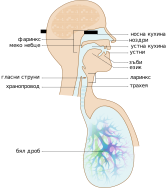
\includegraphics[width=0.48\paperwidth,valign=t]{physics}%
            } \hspace{0.8cm}
            \subfloat[Опростено представяне на вокалния тракт]{%
                \label{fig:physics:1:b}
                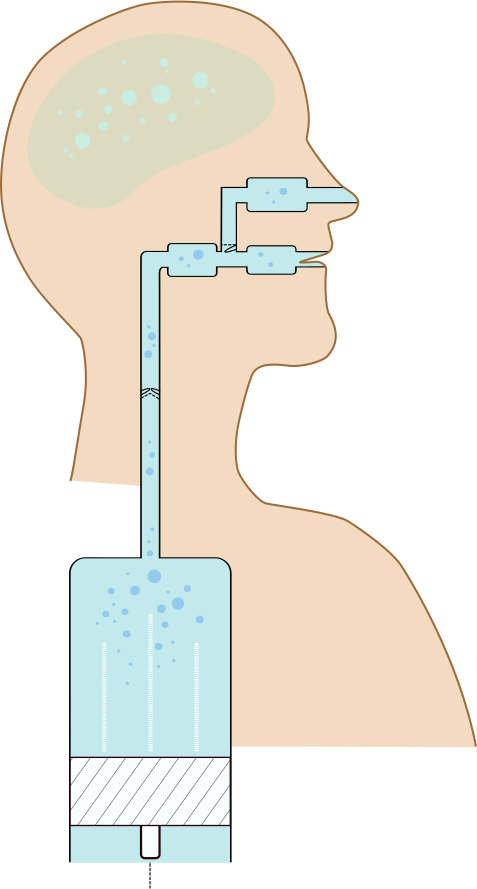
\includegraphics[width=0.28\paperwidth,valign=t]{tubes}%
                \vphantom{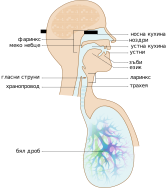
\includegraphics[width=0.48\paperwidth,valign=t]{physics}}%
            }
        \end{changemargin} 
        \caption{Система за производство на реч}%
        \label{fig:physics:1}
    \end{figure}

    Вокален тракт е общото название на кухините над ларинкса (гръкляна), през които минава въздухът при произвеждане на реч.
    При хората той се състои от ларингеална кухина (съдържаща ларинкса и гласните струни), фаринкс, устна кухина и носна кухина, както може да се види на Фигура \autoref{fig:physics:1:a}. Вокалният тракт е отговорен за генериране на различни звуци, като текущата конфигурация на отделните му компоненти определя какъв ще бъде самият звук.
    Според \cite{emotional:shit}, освен от вида на този звук, конфигурацията на вокалния тракт зависи и от емоцията, която изпитва говорещият. Смята се, че емоционалното състояние е пряко свързано с определени промени в организма, например ускорено дишане или мускулно напрежение, а тези промени се отразяват върху произведената реч. Често дори ефектите от тези промени са станали нарицателно за самата емоция. Из българската литература се срещат изречения като ,,страхът стискаше гърлото, задушаваше гласа'' \cite{talev}, а изрази като ,,буца в гърлото'' или ,,пресъхнало гърло'' са навлезли в разговорната реч като асоциации на ,,тъга''. Тъй като изпитваната емоция влияе пряко на конфигурацията на вокалния тракт, бихме искали да извличаме характеристики, които описват тази конфигурация.
    
    Да разгледаме по-подробно класическата постановка, показана на Фигура \autoref{fig:physics:1:b}, която описва цялостна система за производство на реч в по-опростен вариант.
    Речта, всъщност, представлява просто акустичната вълна, получена на края на системата - устни и ноздри - в следствие на изтласкания от белия дроб въздух.

    Белият дроб работи като енергиен източник за тази система - въздушният поток, получен при свиването му от междуребрените мускули и диафрагмата,
    се пропагира нагоре по трахеята и през глотиса (отвора между гласните струни).\\
    Действието на глотиса може да се види най-ясно при произнасяне на гласна. Гласните струни пропускат пропагирания въздух. Тъй като глотисът е стеснение, налягането в него в този момент е по-малко от това в който и да е от двата му края. Съгласно закона на Бернули, в някакъв момент то става толкова ниско, че позволява на гласните струни да се затворят. В следствие се натрупва налягане зад гласните струни заради тласкания от белия дроб въздух, което в някакъв момент ги принуждава да се отворят, и цикълът се повтаря отначало. В резултат се получава осцилиране на гласните струни. Честотата на отварянето и затварянето зависи от анатомични особености като еластичността и големината на гласните струни, налягането в белия дроб и други.\\
    При мъжете тази честота е средно 125 Hz, а при жените - 210 Hz.\\
    Акустичната вълна, която се получава в следствие на осцилацията,
    преминава през вокалния тракт, където се завихря при срещане на прегради като устни и зъби, и в крайна сметка напуска системата през някой от отворите.

    При този процес се губи част от енергията поради различни фактори като съпротивлението на въздуха и поглъщането на вълната от меките и еластични стени на вокалния тракт.

    В зависимост от начина, по който вълната напуска системата, можем да класифицираме произведените звуци по следния начин:

    \begin{enumerate}
        \item Озвучени

        При тези звуци гласните струни осцилират квази-периодично.
        
        \item Проходни (фрикативни) 
        
        При образуването на проходни звуци, вълната среща преграда по пътя си
        (като например зъби, устни) и се получава турболенция, при опита да бъде избутан въздухът през преградата.
        
        \item Преградни (експлозивни)
        
        Те се получават при напълно затворена преграда, зад която се натрупва налягане, което се освобождава рязко чрез отваряне на преградата.
    \end{enumerate}
    
    Обикновено речта, която произнасяме, е разделена на думи, като отделните звукови единици в тях се наричат фонеми. За да се произнесе определена дума,
    вокалният тракт трябва да застане в правилната конфигурация за следващата фонема в думата. Когато
    вокалният тракт се наглася за дадена фонема, настъпват промени, като например стените на устната кухина се приближават или мекото небце, служещо като клапа към носната
    кухина, се затваря. Може да се усети, че при изговаряне на ,,а'' отворът е много по-голям, отколкото при произнасяне на ,,у''.
    Тази промяна влияе върху спектралните свойства на вокалния тракт.
    
    Нека за улеснение си представим, че сме моделирали вокалния тракт с последователност от тръби, за да се абстрахираме от сложната му физическа структура.
    Тогава при смяна на фонемата, се променят дължината и диаметърът на тръбите. Това влияе на времето, за което акустичната вълна ще стигне до края на тръбата,
    и съответно на честотата, на която ще се получи резонанс. Тоест в зависимост от конфигурацията, ще се усилят или затихнат различни честоти, спрямо резонанса.
    Това свойство се нарича честотна пропускливост. Идеята лесно се вижда при свиренето на духови инструменти.

    \begin{figure}[ht]%
    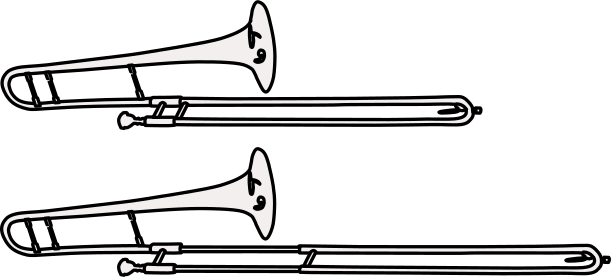
\includegraphics[width=\textwidth]{trombone}%
    \caption{Тромбон}%
    \label{fig:2:1:2}
    \end{figure}

    При тях по някакъв начин се променя изходът на вълната, например отпушване и запушване на дупки, и съответно честотата, на която се
    получава резонанс, тъй като пътят на вълната е скъсен или удължен. Както може да се види на \autoref{fig:2:1:2}, при тромбона буквално се сменя дължината на тръбата,
    което означава, че на вълната ѝ трябва повече време, за да се отрази, тоест резонансът е на по-малка честота и съответно изходящият звук е по-нисък.

    Това значи, че ако знаем как се пропагира вълната по отделните тръби на вокалния тракт и
    какви са спректралните свойства накрая, можем да съдим за текущата му конфигурация.
    В такъв случай, за да изследваме подлежащата емоция при реч е нужно да изследваме тези свойства в достатъчно кратък отрязък от време,
    в който конфигурацията е статична. Обикновено се приема, че този период е между 10 и 20 милисекунди (\cite[стр.~98]{rabiner_schafer78}).
    
    В следващия раздел ще разгледаме как можем да моделираме вокалния тракт с модела на тръбите, за да можем да извлечем спектралните му свойства.
\end{document}